%%%%%%%%%%%%%%%%%%%%%%%%%%%%%%%%%%%%%%%%%%%%%%%%%%%%%%%%%%%%%%%%%%%%%%%%%%%%%%%%%%%%%%%%%%%%%%%%%%%
%%%%%%%%%%%%%%%%%%%%%%%%%%%%%%%%%%%%%%%%%%%%%%%%%%%%%%%%%%%%%%%%%%%%%%%%%%%%%%%%%%%%%%%%%%%%%%%%%%%
%%%%%%%%%%%%%%%%%%%%%%%%%%%%%%%%%%%%%%%%%%%%%%%%%%%%%%%%%%%%%%%%%%%%%%%%%%%%%%%%%%%%%%%%%%%%%%%%%%%
%%%%%%%%%%%%%%%%%%%%%%%%%%%%%%%%%%%%%%%%%%%%%%%%%%%%%%%%%%%%%%%%%%%%%%%%%%%%%%%%%%%%%%%%%%%%%%%%%%%
\chapter{Metodología}

%El presente trabajo resulta de una colaboración con el departamento de Gerontología, dependiente 
%del Instituto de Ciencias de la Salud (ICSA); parte de esta colaboración incluye el acceso a los 
%registros de PSG obtenidos por Vázquez Tagle y colaboradores \cite{VazquezTagle16}. 
%A continuación se expone la metodología de aquél estudio.

\section{Participantes}

Los sujetos fueron elegidos usando un muestreo \textit{no probabilístico por 
conveniencia}\footnote{Lo cual implica que los resultados pueden no deben ser interpolados 
inmediatamente a poblaciones más grandes} bajo los siguientes criterios de inclusión:
\begin{itemize}
\item Edad entre 60 y 85 años
\item Diestros (mano derecha dominante)
\item Sin ansiedad, depresión ni síndromes focales
\item No usar medicamentos o sustancias para dormir
\item Firma de consentimiento informado
\item Voluntario para el registro de PSG
\end{itemize}

Un total de 9 adultos mayores cumplieron los criterios de inclusión. Estos participantes fueron 
sometidos a una batería de pruebas neuropsicológicas para determinar su estado cognoscitivo general 
(Neuropsi, MMSE), descartar cuadros depresivos (GDS, SATS) y cambios en la vida cotidiana (KATZ).
Se concluyó que objetivamente ninguno de ellos padece depresión, y que sus respectivas vidas diarias

Para su análisis, los participantes se dividieron en dos grupos en base a su estado cognoscitivo:
control (CTL) y con Probable Deterioro Cognitivo (PDC). Para la clasificación se dio especial 
atención al puntaje total de Neuropsi estandarizado según edad y escolaridad \cite{Ardila12}, 
criterios que se muestran en la tabla \ref{puntajes}.

\begin{table}
\centering
\caption{Puntajes de corte para Neuropsi}
\begin{tabular}{llrrrr}
\toprule
&&& \multicolumn{3}{c}{Deterioro cognitivo} \\
\cmidrule{4-6} 
Escolaridad & Edad & Normal & Leve & Moderado & Severo\\
\midrule
Nula
& 16 -- 30 & 60 & 45 & 30 & 14 \\
& 31 -- 50 & 68 & 54 & 41 & 28 \\
& 51 -- 65 & 59 & 44 & 28 & 13 \\
& 66 -- 85 & 48 & 34 & 20 & 6 \\
\midrule
1 -- 4 años
& 16 -- 30 & 73 & 58 & 42 & 27 \\
& 31 -- 50 & 81 & 69 & 58 & 46 \\
& 51 -- 65 & 77 & 67 & 57 & 47 \\
& 66 -- 85 & 61 & 46 & 32 & 18 \\
\midrule
5 -- 9 años
& 16 -- 30 &102 & 97 & 86 & 75 \\
& 31 -- 50 &106 &101 & 90 & 79 \\
& 51 -- 65 & 98 & 91 & 79 & 67 \\
& 66 -- 85 & 80 & 72 & 56 & 39 \\
\midrule
10 -- 24 años
& 16 -- 30 &103 & 98 & 87 & 77 \\
& 31 -- 50 &102 & 97 & 88 & 78 \\
& 51 -- 65 & 93 & 88 & 80 & 72 \\
& 66 -- 85 & 78 & 72 & 59 & 46 \\
\bottomrule
\end{tabular}\\
Adaptado de \cite{Ardila12}
\label{puntajes}
\end{table}

%\begin{table}[h]
%\centering
%\begin{tabular}{lcl}
%\toprule
%Grupo & Sujetos & Características \\
%\midrule
%Mn & 4 & Posible Deterioro Cognitivo \\
%Nn & 5 & Sin PDC \\
%ex & 3 & No satisfacen los criterios de inclusión \\
%\bottomrule
%\end{tabular}
%\end{table}

%El grupo ex se conforma de sujeto que incumplen al menos uno de los criterios de inclusión: {FGH} 
%padece parálisis facial y posiblemente daño cerebral (síndromes focales), MGG padece depresión, 
%EMT no califica como adulto mayor por su edad.
%Se efectuaron todos los análisis sobre este grupo, con la finalidad de exhibir las capacidades y
%limitaciones de las técnicas utilizadas; por ello este grupo es ignorado en la sección de 
%resultados pero no en la discusión.

\begin{table}
\caption{Datos generales de los participantes}
\centering
\bordes{1.1}
{\small
\begin{tabular}{llcrrrrrrr}
\toprule
 \phantom{.}&
 & {Sexo} & {Edad} & {Escol.} & {Neuropsi} & {MMSE} & {SATS} & {KATZ} & {GDS} \\
\midrule
\multicolumn{6}{l}{\textbf{Grupo CTL}}\\
&VCR    & F    & 59\pz & 12\pz & 107\pz & 29\pz & 21\pz & 0\pz & 3\pz \\
&MJH    & F    & 72\pz & 9\pz  & 113\pz & 30\pz & 18\pz & 0\pz & 0\pz \\
&JAE    & F    & 78\pz & 5\pz  & 102\pz & 28\pz & 19\pz & 0\pz & 5\pz \\
&GHA    & M    & 65\pz & 9\pz  & 107.5  & 30\pz & 23\pz & 0\pz & 7\pz \\
&MFGR   & F    & 67\pz & 11\pz & 110\pz & 30\pz & 18\pz & 0\pz &      \\
\rowcolor{gris}
&\multicolumn{1}{c}{$\widehat{\mu}$} & 
               & 68.2  & 9.2   & 107.9  & 29.4  & 19.8  & 0.0  & 3.0  \\
\rowcolor{gris}
&\multicolumn{1}{c}{$\widehat{\sigma}$} & 
               & 7.2   & 2.7   & 4.1    & 0.9   & 2.2   & 0.0  & 3.0  \\
\midrulec
%\hline
\multicolumn{6}{l}{\textbf{Grupo PDC}}\\
&CLO    & F    & 68\pz & 5\pz  & 81\pz & 28\pz & 22\pz & 1\pz & 6\pz \\
&RLO    & F    & 63\pz & 9\pz  & 90\pz & 29\pz & 20\pz & 0\pz & 3\pz \\
&RRU    & M    & 69\pz & 9\pz  & 85\pz & 27\pz & 10\pz & 0\pz & 3\pz \\
&JGZ    & M    & 65\pz & 11\pz & 87\pz & 25\pz & 20\pz & 0\pz & 1\pz \\
\rowcolor{gris}
&\multicolumn{1}{c}{$\widehat{\mu}$} & 
              & 66.3   & 8.5   & 85.8  & 27.3  & 18.0  & 0.3  & 3.3  \\
\rowcolor{gris}
&\multicolumn{1}{c}{$\widehat{\sigma}$} & 
              & 2.8    & 2.5   & 3.8   & 1.7   & 5.4   & 0.5  & 2.1  \\
\bottomrulec
\end{tabular} 
}
\label{tab_sujetos}
\end{table}

%\begin{table}
%\centering
%\bordes{1.1}
%\begin{tabular}{c}
%\textbf{Datos generales de los participantes}
%\vspace{1em}
%\end{tabular}
%{\small
%\begin{tabular}{llcrrrrrrr}
%\toprule
% \phantom{.}&
% & {Sexo} & {Edad} & {Escol.} & {Neuropsi} & {MMSE} & {SATS} & {KATZ} & {Gds} \\
%\midrule
%\multicolumn{6}{l}{{Grupo Nn}}\\
%&VCR    & F    & 59\pz & 12\pz & 107\pz & 29\pz & 21\pz & 0\pz & 3\pz \\
%&MJH    & F    & 72\pz & 9\pz  & 113\pz & 30\pz & 18\pz & 0\pz & 0\pz \\
%&JAE    & F    & 78\pz & 5\pz  & 102\pz & 28\pz & 19\pz & 0\pz & 5\pz \\
%&GHA    & M    & 65\pz & 9\pz  & 107.5  & 30\pz & 23\pz & 0\pz & 7\pz \\
%&MFGR   & F    & 67\pz & 11\pz & 110\pz & 30\pz & 18\pz & 0\pz &      \\
%\rowcolor{gris}
%&\multicolumn{1}{c}{$\widehat{\mu}$} & 
%               & 68.2  & 9.2   & 107.9  & 29.4  & 19.8  & 0.0  & 3.0  \\
%\rowcolor{gris}
%&\multicolumn{1}{c}{$\widehat{\sigma}$} & 
%               & 7.2   & 2.7   & 4.1    & 0.9   & 2.2   & 0.0  & 3.0  \\
%\midrulec
%%\hline
%\multicolumn{6}{l}{{Grupo Mn}}\\
%&CLO    & F    & 68\pz & 5\pz  & 81\pz & 28\pz & 22\pz & 1\pz & 6\pz \\
%&RLO    & F    & 63\pz & 9\pz  & 90\pz & 29\pz & 20\pz & 0\pz & 3\pz \\
%&RRU    & M    & 69\pz & 9\pz  & 85\pz & 27\pz & 10\pz & 0\pz & 3\pz \\
%&JGZ    & M    & 65\pz & 11\pz & 87\pz & 25\pz & 20\pz & 0\pz & 1\pz \\
%\rowcolor{gris}
%&\multicolumn{1}{c}{$\widehat{\mu}$} & 
%              & 66.3   & 8.5   & 85.8  & 27.3  & 18.0  & 0.3  & 3.3  \\
%\rowcolor{gris}
%&\multicolumn{1}{c}{$\widehat{\sigma}$} & 
%              & 2.8    & 2.5   & 3.8   & 1.7   & 5.4   & 0.5  & 2.1  \\
%\midrulec
%%\hline
%\multicolumn{6}{l}{{Grupo ex}}\\
%&FGH    & M    & 71\pz   & 9\pz    & 83.5     & 21\pz   & 23\pz   & 0\pz    & 4\pz  \\
%&MGG    & F    & 61\pz   & 9\pz    & 114\pz      & 28\pz   & 29\pz   & 1\pz    & 14\pz \\
%&EMT    & M    & 50\pz   & 22\pz   & 106\pz      & 30\pz   & 15\pz   & 0\pz    & 4\pz  \\
%\bottomrule
%\end{tabular} 
%}
%\label{tab_sujetos}
%\caption{Resultados de las pruebas neuropsicológicas 
%}
%\end{table}

%%%%%%%%%%%%%%%%%%%%%%%%%%%%%%%%%%%%%%%%%%%%%%%%%%%%%%%%%%%%%%%%%%%%%%%%%%%%%%%%%%%%%%%%%%%%%%%%%%%
%%%%%%%%%%%%%%%%%%%%%%%%%%%%%%%%%%%%%%%%%%%%%%%%%%%%%%%%%%%%%%%%%%%%%%%%%%%%%%%%%%%%%%%%%%%%%%%%%%%

\section{Registro del polisomnograma}

Para llevar a cabo el registro, los adultos mayores participantes fueron invitados a acudir a las 
instalaciones de la Clínica Gerontológica de Sueño, ubicada dentro del Instituto de Ciencias de la 
Salud (ICSa) dependiente de la Universidad Autónoma del Estado de Hidalgo. Los participantes 
recibieron instrucciones de realizar una rutina normal de actividades durante la semana que 
precedió al estudio, y se les recomendó no ingerier bebidas alcohólicas o energizantes (como café 
o refresco) durante las 24 horas previas al experimento, y que no durmieran siesta ese día.

Para efectuar el registro se usó un polisomnógrafo Medicid 5 (Neuronic Mexicana).
El protocolo de PSG incluye 19 electrodos de EEG, 4 electrodos de EOG para registrar movimientos 
oculares horizontales y verticales, y 2 electrodos de EMG colocados en los músculos submentonianos 
para registrar la actividad muscular. 
La colocación de electrodos para registrar la actividad EEG se realizó siguiendo las coordenadas 
del Sistema Internacional 10--20 con los lóbulos auriculares como referencia común.
%
La impedancia se mantuvo por debajo de \SI{50}{\micro\ohm}.

Las señales fueron amplificadas analógicamente usando amplificadores de alta ganancia en cadena, 
así mismo fueron filtradas usando filtros de paso de banda: 0.1--100 Hz para EEG, 3--20 Hz para EOG. 
Debido a dificultades técnicas, el registro fue realizado a razón de 512 puntos por segundo (\hz) 
para algunos participantes mientras que se usó 200 puntos por segundo para otros; en ambos casos
se cumple la recomendación de la AASM de un mínimo de 128 Hz.

Los registros fueron segmentados en ventanas de 30 segundos de duración, referidas como 
\textit{épocas}, para ser clasificadas por etapa de sueño según los criterios de la AASM. Esta
clasificación fue llevada a cabo por expertos en sueño de ICSa.

%La clasificación del PSG en fases de sueño se realizó \textit{manualmente} sobre épocas de 30 
%segundos siguiendo los criterios estandarizados de la AASM.

%Debido a un cambio en el polisomnógrafo 
%usado, la frecuencia de muestreo (en Hz) cambia entre sujetos.



\begin{table}
\centering
\caption{Datos generales sobre los registros de PSG}
\bordes{1.2}
{\small
\begin{tabular}{llcllcllr}
\toprule
    \phantom{.}&
    &\multirow{2}{*}{\bordes{1}\begin{tabular}{l}Frecuencia\\ muestreo\end{tabular}}
    \bordes{1.2}
    & \multicolumn{2}{c}{Total} & \phantom{l}   & \multicolumn{3}{c}{MOR*}\\
    \cmidrule{4-5}  \cmidrule{7-9}
    &&          &Puntos  &  Tiempo   &&Puntos  &  Tiempo   &  \% \\
\midrule
\multicolumn{6}{l}{\textbf{Grupo CTL}}\\
&VCR &200       &\ppu 5166000 & \ppu  7:10:30 &&\ppu 438000  &   0:36:30 & 8.5 \\
&MJH &512       &15851520     & \ppu  8:36:00 &&     1950720 &   1:03:30 &12.3 \\
&JAE &512       &13931520     & \ppu  7:33:30 &&     2626560 &   1:25:30 &18.9 \\
&GHA &200       &\ppu 6558000 & \ppu  9:06:00 &&\ppu 330000  &   0:27:30 & 5.0 \\
&MFGR&200       &\ppu 4932000 & \ppu  6:51:00 &&\ppu 570000  &   0:47:30 &11.6 \\

\rowcolor{gris}
&\multicolumn{1}{c}{$\widehat{\mu}$}  
              & &        & \ppu 7:51:30   &&        &   0:52:06 &11.2 \\
\rowcolor{gris}
&\multicolumn{1}{c}{$\widehat{\sigma}$} 
              & &        & \ppu 0:57:36   &&        &   0:23:00 & 5.1 \\
\midrulec

\multicolumn{6}{l}{\textbf{Grupo PDC}}\\
&CLO &512       &    14499840 & \ppu  7:52:00 &&    2027520 &   1:06:00 &14.0 \\
&RLO &512       &    12994560 & \ppu  7:03:00 &&    1520640 &   0:49:30 &11.7 \\
&RRU &200       &\ppu 2484000 & \ppu  3:27:00 &&\ppu 228000  &   0:19:00 & 9.2 \\
&JGZ &512       &    18539520 &      10:03:30 &&\ppu 506880  &   0:16:30 & 2.7 \\

\rowcolor{gris}
&\multicolumn{1}{c}{$\widehat{\mu}$}  
              & &        & \ppu 7:06:23   &&        &   0:37:45 &9.4 \\
\rowcolor{gris}
&\multicolumn{1}{c}{$\widehat{\sigma}$} 
              & &        & \ppu 2:44:55   &&        &   0:24:05 &4.9 \\
\bottomrulec
\end{tabular}\\
*Dado que el sueño MOR aparece fragmentado, se reporta la suma de tales tiempos
}
\label{frecuencias}
\end{table}

%\begin{table}
%\centering
%\bordes{1.2}
%\begin{tabular}{c}
%\textbf{Datos generales sobre los registros de PSG}
%\vspace{1em}
%\end{tabular}
%{\small
%\begin{tabular}{llcrrcrrr}
%\toprule
%    \phantom{.}&
%    &\multirow{2}{*}{\bordes{1}\begin{tabular}{l}Frecuencia\\ muestreo\end{tabular}}
%    \bordes{1.2}
%    & \multicolumn{2}{c}{Total} & \phantom{l}   & \multicolumn{3}{c}{MOR*}\\
%    \cmidrule{4-5}  \cmidrule{7-9}
%    &&          &Puntos  &  Tiempo   &&Puntos  &  Tiempo   &  \% MOR \\
%\midrule
%\multicolumn{6}{l}{{Grupo Nn}}\\
%&VCR &200       & 5166000&   7:10:30 &&438000  &   0:36:30 & 8.5\% \\
%&MJH &512       &15851520&   8:36:00 &&1950720 &   1:03:30 &12.3\% \\
%&JAE &512       &13931520&   7:33:30 &&2626560 &   1:25:30 &18.9\% \\
%&GHA &200       &6558000 &   9:06:00 &&330000  &   0:27:30 & 5.0\% \\
%&MFGR&200       &4932000 &   6:51:00 &&570000  &   0:47:30 &11.6\% \\
%
%\rowcolor{gris}
%&\multicolumn{1}{c}{$\widehat{\mu}$}  
%              & &        & 7:51:30   &&        &   0:52:06 &11.2\% \\
%\rowcolor{gris}
%&\multicolumn{1}{c}{$\widehat{\sigma}$} 
%              & &        & 0:57:36   &&        &   0:23:00 & 5.1\% \\
%\midrulec
%
%\multicolumn{6}{l}{{Grupo Mn}}\\
%&CLO &512       &14499840&   7:52:00 &&2027520 &   1:06:00 &14.0\% \\
%&RLO &512       &12994560&   7:03:00 &&1520640 &   0:49:30 &11.7\% \\
%&RRU &200       &2484000 &   3:27:00 &&228000  &   0:19:00 & 9.2\% \\
%&JGZ &512       &18539520&  10:03:30 &&506880  &   0:16:30 & 2.7\% \\
%
%\rowcolor{gris}
%&\multicolumn{1}{c}{$\widehat{\mu}$}  
%              & &        & 7:06:23   &&        &   0:37:45 &9.4\% \\
%\rowcolor{gris}
%&\multicolumn{1}{c}{$\widehat{\sigma}$} 
%              & &        & 2:44:55   &&        &   0:24:05 &4.9\% \\
%\midrulec
%
%\multicolumn{6}{l}{{Grupo ex}}\\
%&FGH &512       &6220800 &   3:22:30 &&337920  &   0:11:00 & 5.4\% \\
%&MGG &512       &15820800&   8:35:00 &&2549760 &   1:23:00 &16.1\% \\
%&EMT &512       &21857280&  11:51:30 &&721920  &   0:23:30 & 3.3\% \\
%\bottomrule
%\end{tabular}
%}
%\caption{Cantidad de datos registrados para cada sujeto. *Dado que el sueño MOR aparece fragmentado,
%se reporta la suma de tales tiempos.}
%\label{frecuencias}
%\end{table}

%%%%%%%%%%%%%%%%%%%%%%%%%%%%%%%%%%%%%%%%%%%%%%%%%%%%%%%%%%%%%%%%%%%%%%%%%%%%%%%%%%%%%%%%%%%%%%%%%%%
%%%%%%%%%%%%%%%%%%%%%%%%%%%%%%%%%%%%%%%%%%%%%%%%%%%%%%%%%%%%%%%%%%%%%%%%%%%%%%%%%%%%%%%%%%%%%%%%%%%

\section{Aplicación de la prueba de Priestley-Subba Rao}

Los registros digitalizados de PSG fueron convertidos a formato de texto bajo la codificación 
ASCII, a razón de un archivo por cada canal, mientras que las épocas MOR fueron indicadas en 
archivos a parte.
%
Estos datos fueron procesados mediante el software estadístico R \cite{R_citar} tratando cada
canal por separado.

El primer análisis consistió en fragmentar los registros en ventanas independientes de 30 segundos
de duración; cada una de estas ventanas fue clasificada como \textit{estacionaria} si
era posible rechazar ($p<0.05$) la hipótesis de no-estacionariedad usando la prueba de
Priestley-Subba Rao (PSR). 
La prueba de PSR \textit{per se} fue aplicada usando la implementación dentro del paquete 
\texttt{fractal} \cite{R_fractal} bajo la función \texttt{stationarity}.

Los resultados obtenidos se guardaron en archivos de texto para su posterior análisis. Debido
a la gran variabilidad entre el tiempo que los participantes pasaron en sueño MOR, se decidió
basar las comparaciones en proporciones de épocas; por ejemplo, se calculó la proporción de
épocas MOR que son estacionarias para todos los participantes.

%Como se mencionó en secciones anteriores, la prueba PSR está pensada para series de tiempo con 
%media 0, varianza finita y espectro puramente continuo. Se espera que la segunda condición se 
%cumpla para los registros de PSG; las otras dos condiciones fueron \textit{forzadas}, sustrayendo 
%la media y la componente periódica (estimadas) del proceso.
%Para lo anterior, se usó el algoritmo no-paramétrico STL (Seasonal-Trend decomposition using 
%Loess) \cite{Cleveland1990} y que está implementado en R bajo la función \texttt{stl()}.

%La prueba PSR se encuentra implementado en R bajo la función \texttt{stationarity()} del paquete 
%\texttt{fractal}.    
%Los resultados de la prueba PSR, aplicado a todas las épocas contenidas en los registros de PSG,
%fueron almacenados para su análisis posterior.

%El registro de PSG por cada canal fueron analizados por separado, y éstos a su vez fueron divididos
%en épocas de 30 segundos de duración (variando el número de puntos según la frecuencia de muestreo);
%cada época fue clasificada como \textit{estacionaria} si, no pudo rechazarse la hipótesis de 
%estacionariedad usando la prueba PSR ($p < 0.05$).
%La cantidad de épocas estacionarias para cada individuo, durante sueño MOR y NMOR, se muestra en 
%las tablas \ref{total_gpos_total} y \ref{total_gpos_mor}; debido a la gran variabilidad entre los 
%sujetos para la duración del sueño MOR, para el análisis no se consideró el total de épocas sino la 
%proporción de éstas en cada etapa de sueño. 

\begin{figure}
\centering
\begin{lstlisting}[caption={}]
Priestley-Subba Rao stationarity Test for datos
-----------------------------------------------
Samples used              : 3072 
Samples available         : 3069 
Sampling interval         : 1 
SDF estimator             : Multitaper 
  Number of (sine) tapers : 5 
  Centered                : TRUE 
  Recentered              : FALSE 
Number of blocks          : 11 
Block size                : 279 
Number of blocks          : 11 
p-value for T             : 0.4130131 
p-value for I+R           : 0.1787949 
p-value for T+I+R         : 0.1801353 
\end{lstlisting}
\caption[{Resultado típico para la función \texttt{stationarity}}]
{Resultado típico para la función \texttt{stationarity}
%El parámetro \texttt{n.blocks} define la cantidad grupos disjuntos para los cuales se calculará 
%el estimador de la FDE.
%Cabe resaltar el antepenúltimo renglón (\texttt{p-value for T}), según el cual se puede
%aceptar o rechazar la hipótesis de estacionariedad débil. 
%La FDE es referida como 'Spectral Density Function' (SDF).
}
\label{res_psr}
\end{figure}

Posteriormente se repitió la clasificación de épocas estacionarias variando el tamaño de ventana. 
La motivación principal para ello es corroborar el supuesto popular de que si se toman series de 
tiempo \textit{suficiente cortas}, entonces se puede garantizar que son estacionarias. Los tamaños 
de ventana se tomaron de la forma $30 \times 2^{n}$ segundos, por comparabilidad con el tamaño de 
ventana recomendado por la AASM (30 segundos).
%Todas las clasificaciones se realizaron de forma independiente.
%
Esta metodología recrea aquella usada por McEwen \cite{McEwen75}.

%Una práctica común en el análisis de señales electrofisiológicas es el suponer que una serie de 
%tiempo \textit{suficientemente} corta pueda considerarse estacionaria, cuando menos en el sentido
%débil; anteriormente se ha señalado que se trata de un efecto de muestras pequeñas \cite{Melard89},
%y paralelamente se han incorporado a los diseños experimentales motivos para mantener este supuesto
%\cite{Kaiser00}.

%La información obtenida representa, de manera normalizada, cómo la ocurrencia de épocas 
%estacionarias depende de la longitud de las mismas; los tamaños de época se han elegido de la forma 
%$30\times 2^{n}$ segundos, para poder considerar múltiplos y submúltiplos del tamaño de época
%recomendado por la AASM (30 segundos).
%En la figura \ref{cabeza_repoio} se muestra un ejemplo de estos datos, mientras que en el anexo E
%se incluyen gráficos para todos los sujetos.


\begin{figure}
\centering
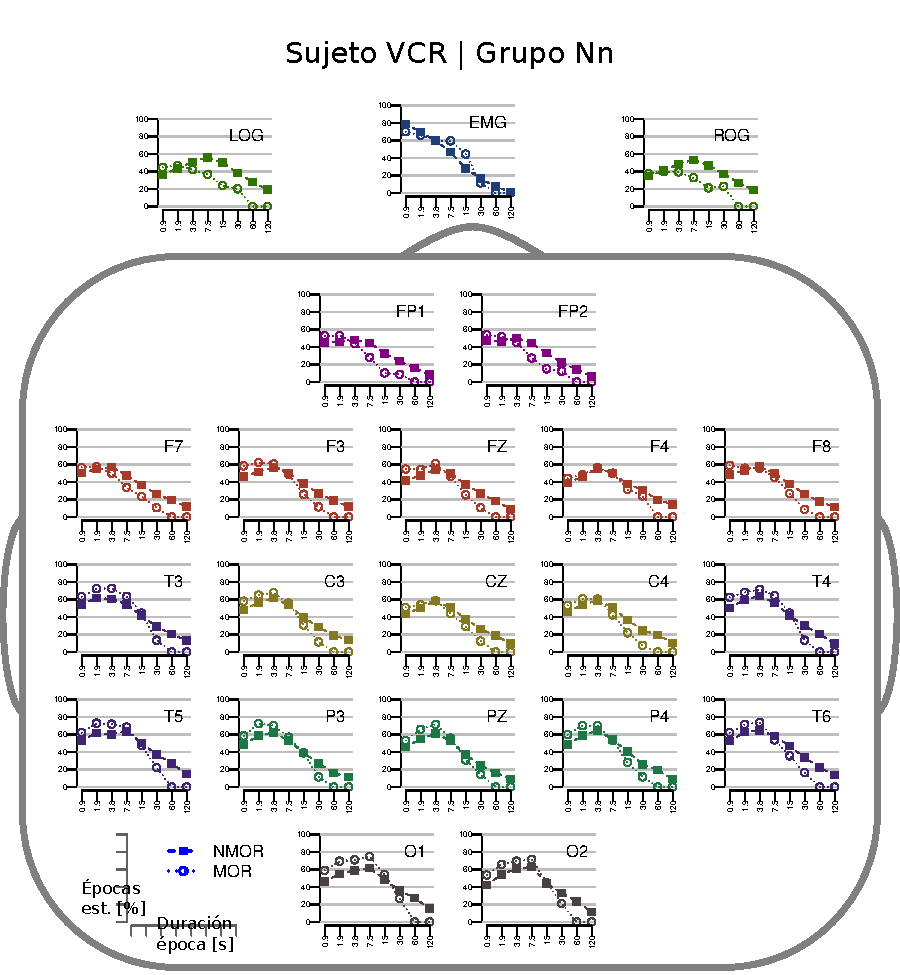
\includegraphics[width=.9\linewidth]{./img_resultados/cabeza_VCR.pdf}
\caption{Porcentajes de épocas estacionarias}
\label{cabeza_repoio}
\end{figure}

\begin{figure}
\centering
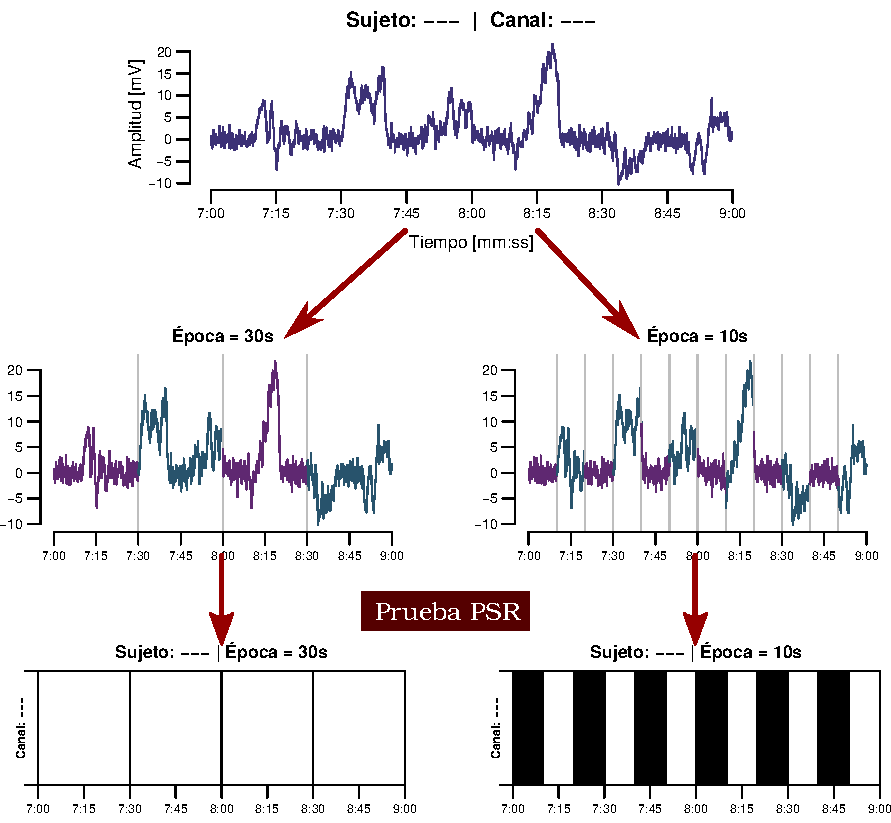
\includegraphics[width=\linewidth]{./img_diagramas/epocas_diferentes_v2.pdf}
\caption{Efecto del tamaño de ventana sobre la clasificación de estacionariedad}
\label{epocas_diferentes}
\end{figure}

Para poder entender la ocurrencia de estacionariedad en diferentes momentos del sueño, las ventanas
se graficaron en el tiempo 

\section{Espectro de potencias}

Se procedió a calcular el espectro integrado de potencias de banda estrecha (bandas delta, theta,
alfa, beta, gamma) para todos los canales.

Cabe destacar que este análisis se decidió \textit{a posteriori} en base a resultados previos [??],
motivo por el cual pareciera ser ligeramente incompatible con los objetivos del trabajo.


%%%%%%%%%%%%%%%%%%%%%%%%%%%%%%%%%%%%%%%%%%%%%%%%%%%%%%%%%%%%%%%%%%%%%%%%%%%%%%%%%%%%%%%%%%%%%%%%%%%
%%%%%%%%%%%%%%%%%%%%%%%%%%%%%%%%%%%%%%%%%%%%%%%%%%%%%%%%%%%%%%%%%%%%%%%%%%%%%%%%%%%%%%%%%%%%%%%%%%%
%%%%%%%%%%%%%%%%%%%%%%%%%%%%%%%%%%%%%%%%%%%%%%%%%%%%%%%%%%%%%%%%%%%%%%%%%%%%%%%%%%%%%%%%%%%%%%%%%%%
%%%%%%%%%%%%%%%%%%%%%%%%%%%%%%%%%%%%%%%%%%%%%%%%%%%%%%%%%%%%%%%%%%%%%%%%%%%%%%%%%%%%%%%%%%%%%%%%%%%